\documentclass[border=5pt]{standalone}
\usepackage{tikz}
\usepackage{amsmath,amssymb,bm}
\usetikzlibrary{arrows.meta, decorations.pathreplacing, calc}

\definecolor{win1}{RGB}{0,80,160}       % dark blue (l=0)
\definecolor{win2}{RGB}{60,130,190}     % mid (l=3)
\definecolor{win3}{RGB}{120,190,230}    % light blue (l=5)

\begin{document}
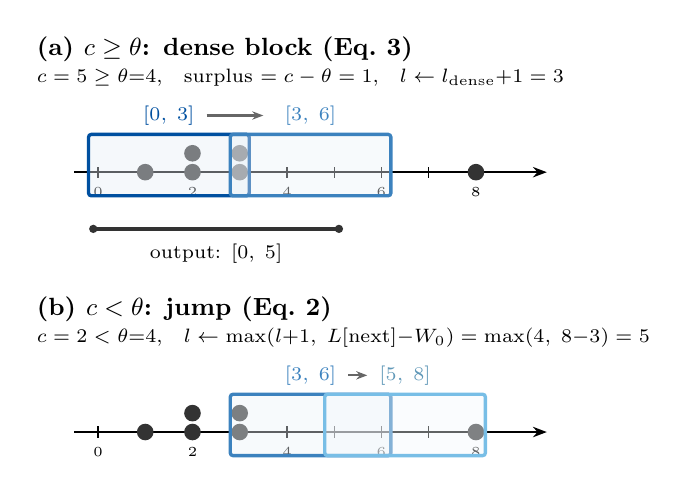
\begin{tikzpicture}[
  scale=0.60,
  every node/.style={font=\small},
  event/.style={circle, fill=black!80, inner sep=0pt, minimum size=6pt},
  timeline/.style={thick, -{Stealth[length=5pt]}},
]

% =====================================================
% (a) Dense block
% =====================================================
\begin{scope}[shift={(0, 0)}]
  \node[font=\bfseries\small, anchor=west] at (-1.5, 2.6)
    {(a) $c \geq \theta$: dense block (Eq.~3)};

  % Annotations
  \node[font=\scriptsize, anchor=west] at (-1.5, 2.0)
    {$c = 5 \geq \theta{=}4$, \;
     surplus $= c - \theta = 1$, \;
     $l \leftarrow l_{\mathrm{dense}}{+}1 = 3$};

  % Timeline
  \draw[timeline] (-0.5, 0) -- (9.5, 0);
  \foreach \x in {0,...,8}
    \draw (\x, -0.12) -- (\x, 0.12);
  \foreach \x in {0,2,...,8}
    \node[below=2pt, font=\tiny] at (\x, 0) {\x};

  % All events
  \node[event] at (1, 0) {};
  \node[event] at (2, 0) {};
  \node[event] at (2, 0.4) {};
  \node[event] at (3, 0) {};
  \node[event] at (3, 0.4) {};
  \node[event] at (8, 0) {};

  % Window l=0: [0, 3] (dark blue)
  \draw[win1, very thick, fill=win1!10, fill opacity=0.4,
    rounded corners=1pt]
    (-0.2, -0.5) rectangle (3.2, 0.8);
  \node[win1, font=\scriptsize] at (1.5, 1.2)
    {$[0,\; 3]$};

  % Arrow between windows
  \draw[-{Stealth[length=4pt]}, thick, black!60]
    (2.3, 1.2) -- (3.5, 1.2);

  % Window l=3: [3, 6] (mid)
  \draw[win2, very thick, fill=win2!10, fill opacity=0.4,
    rounded corners=1pt]
    (2.8, -0.5) rectangle (6.2, 0.8);
  \node[win2, font=\scriptsize] at (4.5, 1.2)
    {$[3,\; 6]$};

  % Dense block output
  \draw[black!80, very thick]
    (-0.1, -1.2) -- (5.1, -1.2);
  \fill[black!80] (-0.1, -1.2) circle (2.5pt);
  \fill[black!80] (5.1, -1.2) circle (2.5pt);
  \node[font=\scriptsize, below=2pt] at (2.5, -1.2)
    {output: $[0,\; 5]$};

\end{scope}

% =====================================================
% (b) Jump
% =====================================================
\begin{scope}[shift={(0, -5.5)}]
  \node[font=\bfseries\small, anchor=west] at (-1.5, 2.6)
    {(b) $c < \theta$: jump (Eq.~2)};

  % Annotations
  \node[font=\scriptsize, anchor=west] at (-1.5, 2.0)
    {$c = 2 < \theta{=}4$, \;
     $l \leftarrow \max(l{+}1,\; L[\mathrm{next}]{-}W_0)
     = \max(4,\; 8{-}3) = 5$};

  % Timeline
  \draw[timeline] (-0.5, 0) -- (9.5, 0);
  \foreach \x in {0,...,8}
    \draw (\x, -0.12) -- (\x, 0.12);
  \foreach \x in {0,2,...,8}
    \node[below=2pt, font=\tiny] at (\x, 0) {\x};

  % All events
  \node[event] at (1, 0) {};
  \node[event] at (2, 0) {};
  \node[event] at (2, 0.4) {};
  \node[event] at (3, 0) {};
  \node[event] at (3, 0.4) {};
  \node[event] at (8, 0) {};

  % Window l=3: [3, 6] (mid)
  \draw[win2, very thick, fill=win2!10, fill opacity=0.4,
    rounded corners=1pt]
    (2.8, -0.5) rectangle (6.2, 0.8);
  \node[win2, font=\scriptsize] at (4.5, 1.2)
    {$[3,\; 6]$};

  % Arrow between windows
  \draw[-{Stealth[length=4pt]}, thick, black!60]
    (5.3, 1.2) -- (5.7, 1.2);

  % Window l=5: [5, 8] (light blue)
  \draw[win3, very thick, fill=win3!10, fill opacity=0.4,
    rounded corners=1pt]
    (4.8, -0.5) rectangle (8.2, 0.8);
  \node[win3!80!black, font=\scriptsize] at (6.5, 1.2)
    {$[5,\; 8]$};

\end{scope}

\end{tikzpicture}
\end{document}
